\def\BBoxR#1#2{
	\vcenter{\hbox{\begin{tikzpicture}[scale=0.20]
	\draw[thick] (0,2) --(2,0) -- (4,2);
	\draw[thick] (0,2) --(2,0) -- (2, -2);	
	\draw[thick] (4,2)--(4,4);
	\draw[thick] (4,6) -- (4,4);	
	\draw (0,2) node[above] {$\scriptstyle{#1}$};
	\draw (4,6) node[above] {$\scriptstyle{#2}$};	
	\draw[fill=white] (4,4) circle (10pt);
	\draw[fill=black] (2,0) circle (10pt);						
	\end{tikzpicture}}}}

\def\CDR#1#2{
	\vcenter{\hbox{\begin{tikzpicture}[scale=0.20]
	\draw[thick] (0,2) --(2,0) -- (4,2);
	\draw[thick] (0,2) --(2,0) -- (2, -2);	
	\draw[thick] (4,2)--(4,4);
	\draw[thick] (4,6) -- (4,4);	
	\draw (0,2) node[above] {$\scriptstyle{#1}$};
	\draw (4,6) node[above] {$\scriptstyle{#2}$};	
	\draw[fill=black] (4,4) circle (10pt);
	\draw[fill=white] (2,0) circle (10pt);						
	\end{tikzpicture}}}}

\def\BBoxL#1#2{
	\vcenter{\hbox{\begin{tikzpicture}[scale=0.20]
	\draw[thick] (0,2) --(2,0) -- (4,2);
	\draw[thick] (0,2) --(2,0) -- (2, -2);	
	\draw[thick] (0,2)--(0,6);
	\draw (0,6) node[above] {$\scriptstyle{#1}$};
	\draw (4,2) node[above] {$\scriptstyle{#2}$};	
	\draw[fill=white] (0,4) circle (10pt);
	\draw[fill=black] (2,0) circle (10pt);			
	\end{tikzpicture}}}}

\def\BBoxLprime#1#2{
	\vcenter{\hbox{\begin{tikzpicture}[scale=0.20]
	\draw[thick] (0,2) --(2,0) -- (4,2);
	\draw[thick] (0,2) --(2,0) -- (2, -2);	
	\draw[thick] (0,2)--(0,6);
	\draw (0,6) node[above] {$\scriptstyle{#1}$};
	\draw (4,2) node[above] {$\scriptstyle{#2}$};	
	\draw[thin, fill=black] (1.5, 0) -- (2, 0.5) -- (2.5,0) -- (2, -0.5) -- cycle;	
	\draw[thin, fill=white] (-0.5, 4) -- (0, 4.5) -- (0.5,4) -- (0, 3.5) -- cycle;
	\end{tikzpicture}}}}

\def\CDL#1#2{
	\vcenter{\hbox{\begin{tikzpicture}[scale=0.20]
	\draw[thick] (0,2) --(2,0) -- (4,2);
	\draw[thick] (0,2) --(2,0) -- (2, -2);	
	\draw[thick] (0,2)--(0,6);
	\draw (0,6) node[above] {$\scriptstyle{#1}$};
	\draw (4,2) node[above] {$\scriptstyle{#2}$};	
	\draw[fill=black] (0,4) circle (10pt);
	\draw[fill=white] (2,0) circle (10pt);			
	\end{tikzpicture}}}}
	
\def\CDLprime#1#2{
	\vcenter{\hbox{\begin{tikzpicture}[scale=0.20]
	\draw[thick] (0,2) --(2,0) -- (4,2);
	\draw[thick] (0,2) --(2,0) -- (2, -2);	
	\draw[thick] (0,2)--(0,6);
	\draw (0,6) node[above] {$\scriptstyle{#1}$};
	\draw (4,2) node[above] {$\scriptstyle{#2}$};	
	\draw[thin, fill=white] (1.5, 0) -- (2, 0.5) -- (2.5,0) -- (2, -0.5) -- cycle;	
	\draw[thin, fill=black] (-0.5, 4) -- (0, 4.5) -- (0.5,4) -- (0, 3.5) -- cycle;
	\end{tikzpicture}}}}	

\def\DC#1#2{
	\vcenter{\hbox{\begin{tikzpicture}[scale=0.20]
	\draw[thick] (0,2) --(2,0) -- (4,2);
	\draw[thick] (0,2) --(2,0) -- (2, -4);	
	\draw (0,2) node[above] {$\scriptstyle{#1}$};
	\draw (4,2) node[above] {$\scriptstyle{#2}$};	
	\draw[fill=black] (2,-2) circle (10pt);		
	\draw[fill=white] (2,0) circle (10pt);			
	\end{tikzpicture}}}}
	
\def\DCprime#1#2{
	\vcenter{\hbox{\begin{tikzpicture}[scale=0.20]
	\draw[thick] (0,2) --(2,0) -- (4,2);
	\draw[thick] (0,2) --(2,0) -- (2, -4);	
	\draw (0,2) node[above] {$\scriptstyle{#1}$};
	\draw (4,2) node[above] {$\scriptstyle{#2}$};	
	\draw[thin, fill=white] (1.5, 0) -- (2, 0.5) -- (2.5,0) -- (2, -0.5) -- cycle;	
	\draw[thin, fill=black] (1.5, -2) -- (2, -1.5) -- (2.5,-2) -- (2, -2.5) -- cycle;	
	\end{tikzpicture}}}}	

\def\BoxB#1#2{
	\vcenter{\hbox{\begin{tikzpicture}[scale=0.20]
	\draw[thick] (0,2) --(2,0) -- (4,2);
	\draw[thick] (0,2) --(2,0) -- (2, -4);	
	\draw (0,2) node[above] {$\scriptstyle{#1}$};
	\draw (4,2) node[above] {$\scriptstyle{#2}$};	
	\draw[fill=white] (2,-2) circle (10pt);		
	\draw[fill=black] (2,0) circle (10pt);			
	\end{tikzpicture}}}}

\def\BoxBprime#1#2{
	\vcenter{\hbox{\begin{tikzpicture}[scale=0.20]
	\draw[thick] (0,2) --(2,0) -- (4,2);
	\draw[thick] (0,2) --(2,0) -- (2, -4);	
	\draw (0,2) node[above] {$\scriptstyle{#1}$};
	\draw (4,2) node[above] {$\scriptstyle{#2}$};	
	\draw[thin, fill=black] (1.5, 0) -- (2, 0.5) -- (2.5,0) -- (2, -0.5) -- cycle;	
	\draw[thin, fill=white] (1.5, -2) -- (2, -1.5) -- (2.5,-2) -- (2, -2.5) -- cycle;	
	\end{tikzpicture}}}}

\def\CB#1#2#3{
	\vcenter{\hbox{\begin{tikzpicture}[scale=0.2]
	\draw[thick] (0,6) -- (4,2) -- (4,0);
	\draw[thick] (4,6) -- (2,4)--(4,2)--(6,4);
	\draw (0,6) node[above] {$\scriptstyle{#1}$};
	\draw (4,6) node[above] {$\scriptstyle{#2}$};	
	\draw (6,4) node[above] {$\scriptstyle{#3}$};				
	\draw[fill=white] (4,2) circle (10pt);	
	\draw[fill=black] (2,4) circle (10pt);	
	\end{tikzpicture}}}}

\def\CBprime#1#2#3{
	\vcenter{\hbox{\begin{tikzpicture}[scale=0.2]
	\draw[thick] (0,6) -- (4,2) -- (4,0);
	\draw[thick] (4,6) -- (2,4)--(4,2)--(6,4);
	\draw (0,6) node[above] {$\scriptstyle{#1}$};
	\draw (4,6) node[above] {$\scriptstyle{#2}$};	
	\draw (6,4) node[above] {$\scriptstyle{#3}$};				
	\draw[thin, fill=white] (3.5, 2) -- (4, 2.5) -- (4.5,2) -- (4, 1.5) -- cycle;		
	\draw[thin, fill=black] (1.5, 4) -- (2, 4.5) -- (2.5,4) -- (2, 3.5) -- cycle;			
	\end{tikzpicture}}}}

\def\BC#1#2#3{
	\vcenter{\hbox{\begin{tikzpicture}[scale=0.2]
	\draw[thick] (0,6) -- (4,2) -- (4,0);
	\draw[thick] (4,6) -- (2,4)--(4,2)--(6,4);
	\draw (0,6) node[above] {$\scriptstyle{#1}$};
	\draw (4,6) node[above] {$\scriptstyle{#2}$};	
	\draw (6,4) node[above] {$\scriptstyle{#3}$};				
	\draw[fill=black] (4,2) circle (10pt);	
	\draw[fill=white] (2,4) circle (10pt);	
	\end{tikzpicture}}}}

\def\BCprime#1#2#3{
	\vcenter{\hbox{\begin{tikzpicture}[scale=0.2]
	\draw[thick] (0,6) -- (4,2) -- (4,0);
	\draw[thick] (4,6) -- (2,4)--(4,2)--(6,4);
	\draw (0,6) node[above] {$\scriptstyle{#1}$};
	\draw (4,6) node[above] {$\scriptstyle{#2}$};	
	\draw (6,4) node[above] {$\scriptstyle{#3}$};				
	\draw[thin, fill=black] (3.5, 2) -- (4, 2.5) -- (4.5,2) -- (4, 1.5) -- cycle;		
	\draw[thin, fill=white] (1.5, 4) -- (2, 4.5) -- (2.5,4) -- (2, 3.5) -- cycle;			
	\end{tikzpicture}}}}

\def\BoxD{
	\vcenter{\hbox{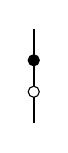
\begin{tikzpicture}[scale=0.2]
	\draw[thick] (2,4) -- (2,6);
	\draw[thick] (2,2) -- (2,4);
	\draw[thick] (2,2) -- (2,0);
	\draw[fill=black] (2,4) circle (10pt);	
	\draw[fill=white] (2,2) circle (10pt);	
	\end{tikzpicture}}}}

\def\BoxDprime{
	\vcenter{\hbox{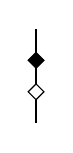
\begin{tikzpicture}[scale=0.2]
	\draw[thick] (2,4) -- (2,6);
	\draw[thick] (2,2) -- (2,4);
	\draw[thick] (2,2) -- (2,0);
	\draw[thin, fill=white] (1.5, 2) -- (2, 2.5) -- (2.5,2) -- (2, 1.5) -- cycle;	
	\draw[thin, fill=black] (1.5, 4) -- (2, 4.5) -- (2.5,4) -- (2, 3.5) -- cycle;	
	\end{tikzpicture}}}}

\def\DBox{
	\vcenter{\hbox{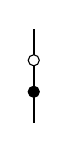
\begin{tikzpicture}[scale=0.2]
	\draw[thick] (2,4) -- (2,6);
	\draw[thick] (2,2) -- (2,4);
	\draw[thick] (2,2) -- (2,0);
	\draw[fill=white] (2,4) circle (10pt);	
	\draw[fill=black] (2,2) circle (10pt);	
	\end{tikzpicture}}}}

\def\DBoxprime{
	\vcenter{\hbox{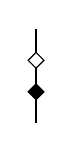
\begin{tikzpicture}[scale=0.2]
	\draw[thick] (2,4) -- (2,6);
	\draw[thick] (2,2) -- (2,4);
	\draw[thick] (2,2) -- (2,0);
	\draw[thin, fill=black] (1.5, 2) -- (2, 2.5) -- (2.5,2) -- (2, 1.5) -- cycle;	
	\draw[thin, fill=white] (1.5, 4) -- (2, 4.5) -- (2.5,4) -- (2, 3.5) -- cycle;	
	\end{tikzpicture}}}}

\def\RMBox#1#2#3{
	\vcenter{\hbox{\begin{tikzpicture}[scale=0.2]
	\draw[thick] (6,6) -- (2,2) -- (2,0);
	\draw[thick] (2,6) -- (4,4)--(2,2)--(0,4);
	\draw (2,6) node[above] {$\scriptstyle{#2}$};
	\draw (6,6) node[above] {$\scriptstyle{#3}$};	
	\draw (0,4) node[above] {$\scriptstyle{#1}$};	
	\draw[fill=white] (4,4) circle (10pt);					
	\end{tikzpicture}}}}

\def\LMBox#1#2#3{
	\vcenter{\hbox{\begin{tikzpicture}[scale=0.2]
	\draw[thick] (0,6) -- (4,2) -- (4,0);
	\draw[thick] (4,6) -- (2,4)--(4,2)--(6,4);
	\draw (0,6) node[above] {$\scriptstyle{#1}$};
	\draw (4,6) node[above] {$\scriptstyle{#2}$};	
	\draw (6,4) node[above] {$\scriptstyle{#3}$};				
	\draw[fill=white] (2,4) circle (10pt);		
	\end{tikzpicture}}}}

\def\LMBoxprime#1#2#3{
	\vcenter{\hbox{\begin{tikzpicture}[scale=0.2]
	\draw[thick] (0,6) -- (4,2) -- (4,0);
	\draw[thick] (4,6) -- (2,4)--(4,2)--(6,4);
	\draw (0,6) node[above] {$\scriptstyle{#1}$};
	\draw (4,6) node[above] {$\scriptstyle{#2}$};	
	\draw (6,4) node[above] {$\scriptstyle{#3}$};	
	\draw[thin] (3.5, 2) -- (4, 2.5) -- (4.5,2) -- (4, 1.5) -- cycle;					
	\draw[thin, fill=white] (1.5, 4) -- (2, 4.5) -- (2.5,4) -- (2, 3.5) -- cycle;												
	\end{tikzpicture}}}}

\def\LCCprime#1#2#3{
	\vcenter{\hbox{\begin{tikzpicture}[scale=0.2]
	\draw[thick] (0,6) -- (4,2) -- (4,0);
	\draw[thick] (4,6) -- (2,4)--(4,2)--(6,4);
	\draw (0,6) node[above] {$\scriptstyle{#1}$};
	\draw (4,6) node[above] {$\scriptstyle{#2}$};	
	\draw (6,4) node[above] {$\scriptstyle{#3}$};	
	\draw[thin, fill=white] (3.5, 2) -- (4, 2.5) -- (4.5,2) -- (4, 1.5) -- cycle;					
	\draw[thin, fill=white] (1.5, 4) -- (2, 4.5) -- (2.5,4) -- (2, 3.5) -- cycle;												
	\end{tikzpicture}}}}

\def\LBoxM#1#2#3{
	\vcenter{\hbox{\begin{tikzpicture}[scale=0.2]
	\draw[thick] (0,6) -- (4,2) -- (4,0);
	\draw[thick] (4,6) -- (2,4)--(4,2)--(6,4);
	\draw (0,6) node[above] {$\scriptstyle{#1}$};
	\draw (4,6) node[above] {$\scriptstyle{#2}$};	
	\draw (6,4) node[above] {$\scriptstyle{#3}$};				
	\draw[fill=white] (4,2) circle (10pt);
	\end{tikzpicture}}}}


\def\LBoxMprime#1#2#3{
	\vcenter{\hbox{\begin{tikzpicture}[scale=0.2]
	\draw[thick] (0,6) -- (4,2) -- (4,0);
	\draw[thick] (4,6) -- (2,4)--(4,2)--(6,4);
	\draw (0,6) node[above] {$\scriptstyle{#1}$};
	\draw (4,6) node[above] {$\scriptstyle{#2}$};	
	\draw (6,4) node[above] {$\scriptstyle{#3}$};				
	\draw[thin, fill=white] (3.5, 2) -- (4, 2.5) -- (4.5,2) -- (4, 1.5) -- cycle;					
	\draw[thin] (1.5, 4) -- (2, 4.5) -- (2.5,4) -- (2, 3.5) -- cycle;												
	\end{tikzpicture}}}}
	
\def\MBoxR#1#2{
	\vcenter{\hbox{\begin{tikzpicture}[scale=0.20]
	\draw[thick] (0,2) --(2,0) -- (4,2);
	\draw[thick] (0,2) --(2,0) -- (2, -2);	
	\draw[thick] (4,2)--(4,4);
	\draw[thick] (4,6) -- (4,4);	
	\draw (0,2) node[above] {$\scriptstyle{#1}$};
	\draw (4,6) node[above] {$\scriptstyle{#2}$};	
	\draw[fill=white] (4,4) circle (10pt);		
	\end{tikzpicture}}}}

\def\MBoxBox#1#2{
	\vcenter{\hbox{\begin{tikzpicture}[scale=0.20]
	\draw[thick] (0,2) --(2,0) -- (4,2);
	\draw[thick] (0,2) --(2,0) -- (2, -2);	
	\draw[thick] (4,2)--(4,6);
	\draw[thick] (0,2)--(0,6);	
	\draw (0,6) node[above] {$\scriptstyle{#1}$};
	\draw (4,6) node[above] {$\scriptstyle{#2}$};	
	\draw[fill=white] (4,4) circle (10pt);	
	\draw[fill=white] (0,4) circle (10pt);			
	\end{tikzpicture}}}}

\def\CBoxR#1#2{
	\vcenter{\hbox{\begin{tikzpicture}[scale=0.20]
	\draw[thick] (0,2) --(2,0) -- (4,2);
	\draw[thick] (0,2) --(2,0) -- (2, -2);	
	\draw[thick] (4,2)--(4,4);
	\draw[thick] (4,6) -- (4,4);	
	\draw (0,2) node[above] {$\scriptstyle{#1}$};
	\draw (4,6) node[above] {$\scriptstyle{#2}$};	
	\draw[fill=white] (4,4) circle (10pt);	
	\draw[fill=white] (2,0) circle (10pt);			
	\end{tikzpicture}}}}

\def\MBoxBoxR#1#2{
	\vcenter{\hbox{\begin{tikzpicture}[scale=0.20]
	\draw[thick] (0,2) --(2,0) -- (4,2);
	\draw[thick] (0,2) --(2,0) -- (2, -2);	
	\draw[thick] (4,2)--(4,4);
	\draw[thick] (4,8) -- (4,4);	
	\draw (0,2) node[above] {$\scriptstyle{#1}$};
	\draw (4,8) node[above] {$\scriptstyle{#2}$};	
	\draw[fill=white] (4,4) circle (10pt);	
	\draw[fill=white] (4,6) circle (10pt);				
	\end{tikzpicture}}}}

\def\MBoxBoxL#1#2{
	\vcenter{\hbox{\begin{tikzpicture}[scale=0.20]
	\draw[thick] (0,2) --(2,0) -- (4,2);
	\draw[thick] (0,2) --(2,0) -- (2, -2);	
	\draw[thick] (0,2)--(0,8);
	\draw (0,8) node[above] {$\scriptstyle{#1}$};	
	\draw (4,2) node[above] {$\scriptstyle{#2}$};
	\draw[fill=white] (0,4) circle (10pt);	
	\draw[fill=white] (0,6) circle (10pt);				
	\end{tikzpicture}}}}

\def\MBoxRsusp#1#2{
	\vcenter{\hbox{\begin{tikzpicture}[scale=0.20]
	\draw[thick] (0,2) --(2,0) -- (4,2);
	\draw[thick] (0,2) --(2,0) -- (2, -2);	
	\draw[thick] (4,2)--(4,4);
	\draw[thick] (4,6) -- (4,4);	
	\draw (0,2) node[above] {$\scriptstyle{#1}$};
	\draw (4,6) node[above] {$\scriptstyle{#2}$};	
	\draw (2,0) node[left] {$\scriptstyle{s}$};
	\draw (4,4) node[left] {$\scriptstyle{s}$};				
	\draw[fill=white] (4,4) circle (10pt);		
	\end{tikzpicture}}}}

\def\MBoxL#1#2{
	\vcenter{\hbox{\begin{tikzpicture}[scale=0.20]
	\draw[thick] (0,2) --(2,0) -- (4,2);
	\draw[thick] (0,2) --(2,0) -- (2, -2);	
	\draw[thick] (0,2)--(0,6);
	\draw (0,6) node[above] {$\scriptstyle{#1}$};
	\draw (4,2) node[above] {$\scriptstyle{#2}$};	
	\draw[fill=white] (0,4) circle (10pt);		
	\end{tikzpicture}}}}

\def\CBoxL#1#2{
	\vcenter{\hbox{\begin{tikzpicture}[scale=0.20]
	\draw[thick] (0,2) --(2,0) -- (4,2);
	\draw[thick] (0,2) --(2,0) -- (2, -2);	
	\draw[thick] (0,2)--(0,6);
	\draw (0,6) node[above] {$\scriptstyle{#1}$};
	\draw (4,2) node[above] {$\scriptstyle{#2}$};	
	\draw[fill=white] (0,4) circle (10pt);		
	\draw[fill=white] (2,0) circle (10pt);			
	\end{tikzpicture}}}}
	
\def\MBoxLsusp#1#2{
	\vcenter{\hbox{\begin{tikzpicture}[scale=0.20]
	\draw[thick] (0,2) --(2,0) -- (4,2);
	\draw[thick] (0,2) --(2,0) -- (2, -2);	
	\draw[thick] (0,2)--(0,6);
	\draw (0,6) node[above] {$\scriptstyle{#1}$};
	\draw (4,2) node[above] {$\scriptstyle{#2}$};	
	\draw (2,0) node[left] {$\scriptstyle{s}$};
	\draw (0,4) node[left] {$\scriptstyle{s}$};				
	\draw[fill=white] (0,4) circle (10pt);		
	\end{tikzpicture}}}}	

\def\MBoxLprime#1#2{
	\vcenter{\hbox{\begin{tikzpicture}[scale=0.20]
	\draw[thick] (0,2) --(2,0) -- (4,2);
	\draw[thick] (0,2) --(2,0) -- (2, -2);	
	\draw[thick] (0,2)--(0,6);
	\draw (0,6) node[above] {$\scriptstyle{#1}$};
	\draw (4,2) node[above] {$\scriptstyle{#2}$};	
	\draw[thin] (1.5, 0) -- (2, 0.5) -- (2.5,0) -- (2, -0.5) -- cycle;	
	\draw[thin, fill=white] (-0.5, 4) -- (0, 4.5) -- (0.5,4) -- (0, 3.5) -- cycle;	
	\end{tikzpicture}}}}

\def\CBoxLprime#1#2{
	\vcenter{\hbox{\begin{tikzpicture}[scale=0.20]
	\draw[thick] (0,2) --(2,0) -- (4,2);
	\draw[thick] (0,2) --(2,0) -- (2, -2);	
	\draw[thick] (0,2)--(0,6);
	\draw (0,6) node[above] {$\scriptstyle{#1}$};
	\draw (4,2) node[above] {$\scriptstyle{#2}$};	
	\draw[thin, fill=white] (1.5, 0) -- (2, 0.5) -- (2.5,0) -- (2, -0.5) -- cycle;	
	\draw[thin, fill=white] (-0.5, 4) -- (0, 4.5) -- (0.5,4) -- (0, 3.5) -- cycle;	
	\end{tikzpicture}}}}

\def\BoxM#1#2{
	\vcenter{\hbox{\begin{tikzpicture}[scale=0.20]
	\draw[thick] (0,2) --(2,0) -- (4,2);
	\draw[thick] (0,2) --(2,0) -- (2, -4);	
	\draw (0,2) node[above] {$\scriptstyle{#1}$};
	\draw (4,2) node[above] {$\scriptstyle{#2}$};	
	\draw[fill=white] (2,-2) circle (10pt);		
	\end{tikzpicture}}}}

\def\BoxC#1#2{
	\vcenter{\hbox{\begin{tikzpicture}[scale=0.20]
	\draw[thick] (0,2) --(2,0) -- (4,2);
	\draw[thick] (0,2) --(2,0) -- (2, -4);	
	\draw (0,2) node[above] {$\scriptstyle{#1}$};
	\draw (4,2) node[above] {$\scriptstyle{#2}$};	
	\draw[fill=white] (2,-2) circle (10pt);	
	\draw[fill=white] (2,0) circle (10pt);			
	\end{tikzpicture}}}}

\def\BoxBoxM#1#2{
	\vcenter{\hbox{\begin{tikzpicture}[scale=0.20]
	\draw[thick] (0,2) --(2,0) -- (4,2);
	\draw[thick] (0,2) --(2,0) -- (2, -6);	
	\draw (0,2) node[above] {$\scriptstyle{#1}$};
	\draw (4,2) node[above] {$\scriptstyle{#2}$};	
	\draw[fill=white] (2,-2) circle (10pt);	
	\draw[fill=white] (2,-4) circle (10pt);	
	\end{tikzpicture}}}}

\def\BoxMBoxL#1#2{
	\vcenter{\hbox{\begin{tikzpicture}[scale=0.20]
	\draw[thick] (0,2) --(2,0) -- (4,2);
	\draw[thick] (0,2) --(2,0) -- (2, -4);	
	\draw[thick] (0,2)--(0,6);	
	\draw (0,6) node[above] {$\scriptstyle{#1}$};
	\draw (4,2) node[above] {$\scriptstyle{#2}$};	
	\draw[fill=white] (2,-2) circle (10pt);		
	\draw[fill=white] (0,4) circle (10pt);			
	\end{tikzpicture}}}}

\def\BoxMBoxR#1#2{
	\vcenter{\hbox{\begin{tikzpicture}[scale=0.20]
	\draw[thick] (0,2) --(2,0) -- (4,2);
	\draw[thick] (0,2) --(2,0) -- (2, -4);	
	\draw[thick] (4,2)--(4,6);	
	\draw (4,6) node[above] {$\scriptstyle{#2}$};
	\draw (0,2) node[above] {$\scriptstyle{#1}$};	
	\draw[fill=white] (2,-2) circle (10pt);		
	\draw[fill=white] (4,4) circle (10pt);			
	\end{tikzpicture}}}}

\def\BoxMsusp#1#2{
	\vcenter{\hbox{\begin{tikzpicture}[scale=0.20]
	\draw[thick] (0,2) --(2,0) -- (4,2);
	\draw[thick] (0,2) --(2,0) -- (2, -4);	
	\draw (0,2) node[above] {$\scriptstyle{#1}$};
	\draw (4,2) node[above] {$\scriptstyle{#2}$};
	\draw (2,0) node[left] {$\scriptstyle{s}$};
	\draw (2,-2) node[left] {$\scriptstyle{s}$};				
	\draw[fill=white] (2,-2) circle (10pt);		
	\end{tikzpicture}}}}

\def\BoxMprime#1#2{
	\vcenter{\hbox{\begin{tikzpicture}[scale=0.20]
	\draw[thick] (0,2) --(2,0) -- (4,2);
	\draw[thick] (0,2) --(2,0) -- (2, -4);	
	\draw (0,2) node[above] {$\scriptstyle{#1}$};
	\draw (4,2) node[above] {$\scriptstyle{#2}$};	
	\draw[thin] (1.5, 0) -- (2, 0.5) -- (2.5,0) -- (2, -0.5) -- cycle;	
	\draw[thin, fill=white] (1.5, -2) -- (2, -1.5) -- (2.5,-2) -- (2, -2.5) -- cycle;		
	\end{tikzpicture}}}}

\def\BoxCprime#1#2{
	\vcenter{\hbox{\begin{tikzpicture}[scale=0.20]
	\draw[thick] (0,2) --(2,0) -- (4,2);
	\draw[thick] (0,2) --(2,0) -- (2, -4);	
	\draw (0,2) node[above] {$\scriptstyle{#1}$};
	\draw (4,2) node[above] {$\scriptstyle{#2}$};	
	\draw[thin, fill=white] (1.5, 0) -- (2, 0.5) -- (2.5,0) -- (2, -0.5) -- cycle;	
	\draw[thin, fill=white] (1.5, -2) -- (2, -1.5) -- (2.5,-2) -- (2, -2.5) -- cycle;		
	\end{tikzpicture}}}}

\def\CC#1#2{
	\vcenter{\hbox{\begin{tikzpicture}[scale=0.2]
	\draw[thick] (0,4) -- (2,2);
	\draw[thick] (4,4) -- (2,2);
	\draw[thick] (2,2) -- (2,0);
	\draw[fill=white] (2,2) circle (10pt);
	\draw (0,4) node[above] {$\scriptstyle{#1}$};
	\draw (4,4) node[above] {$\scriptstyle{#2}$};		
	\end{tikzpicture}}}}

\def\CCsusp#1#2{
	\vcenter{\hbox{\begin{tikzpicture}[scale=0.2]
	\draw[thick] (0,4) -- (2,2);
	\draw[thick] (4,4) -- (2,2);
	\draw[thick] (2,2) -- (2,0);
	\draw[fill=white] (2,2) circle (10pt);
	\draw (0,4) node[above] {$\scriptstyle{#1}$};
	\draw (4,4) node[above] {$\scriptstyle{#2}$};	
	\draw (2,2) node[left] {$\scriptstyle{s}$};			
	\end{tikzpicture}}}}

\def\BOX{
	\vcenter{\hbox{\begin{tikzpicture}[scale=0.15]
	\draw[thick] (2,2) -- (2,4);
	\draw[thick] (2,2) -- (2,0);
	\draw[fill=white] (2,2) circle (10pt);	
	\end{tikzpicture}}}}

\def\BOXprime{
	\vcenter{\hbox{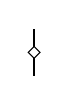
\begin{tikzpicture}[scale=0.15]
	\draw[thick] (2,2) -- (2,4);
	\draw[thick] (2,2) -- (2,0);
	\draw[thin, fill=white] (1.5, 2) -- (2, 2.5) -- (2.5,2) -- (2, 1.5) -- cycle;	
	\end{tikzpicture}}}}

\def\Cprime{
	\vcenter{\hbox{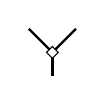
\begin{tikzpicture}[scale=0.15]
	\draw[thick] (0,4) -- (2,2);
	\draw[thick] (4,4) -- (2,2);
	\draw[thick] (2,2) -- (2,0);
	\draw[thin, fill=white] (1.5, 2) -- (2, 2.5) -- (2.5,2) -- (2, 1.5) -- cycle;	
	\end{tikzpicture}}}}

\def\C{
	\vcenter{\hbox{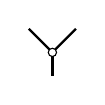
\begin{tikzpicture}[scale=0.15]
	\draw[thick] (0,4) -- (2,2);
	\draw[thick] (4,4) -- (2,2);
	\draw[thick] (2,2) -- (2,0);
	\draw[fill=white] (2,2) circle (10pt);
	\end{tikzpicture}}}}

\def\BDR#1#2{
	\vcenter{\hbox{\begin{tikzpicture}[scale=0.20]
	\draw[thick] (0,2) --(2,0) -- (4,2);
	\draw[thick] (0,2) --(2,0) -- (2, -2);	
	\draw[thick] (4,2)--(4,4);
	\draw[thick] (4,6) -- (4,4);	
	\draw (0,2) node[above] {$\scriptstyle{#1}$};
	\draw (4,6) node[above] {$\scriptstyle{#2}$};	
	\draw[fill=black] (4,4) circle (10pt);
	\draw[fill=black] (2,0) circle (10pt);						
	\end{tikzpicture}}}}

\def\BDL#1#2{
	\vcenter{\hbox{\begin{tikzpicture}[scale=0.20]
	\draw[thick] (0,2) --(2,0) -- (4,2);
	\draw[thick] (0,2) --(2,0) -- (2, -2);	
	\draw[thick] (0,2)--(0,6);
	\draw (0,6) node[above] {$\scriptstyle{#1}$};
	\draw (4,2) node[above] {$\scriptstyle{#2}$};	
	\draw[fill=black] (0,4) circle (10pt);
	\draw[fill=black] (2,0) circle (10pt);			
	\end{tikzpicture}}}}

\def\BDLprime#1#2{
	\vcenter{\hbox{\begin{tikzpicture}[scale=0.20]
	\draw[thick] (0,2) --(2,0) -- (4,2);
	\draw[thick] (0,2) --(2,0) -- (2, -2);	
	\draw[thick] (0,2)--(0,6);
	\draw (0,6) node[above] {$\scriptstyle{#1}$};
	\draw (4,2) node[above] {$\scriptstyle{#2}$};	
	\draw[thin, fill=black] (1.5, 0) -- (2, 0.5) -- (2.5,0) -- (2, -0.5) -- cycle;	
	\draw[thin, fill=black] (-0.5, 4) -- (0, 4.5) -- (0.5,4) -- (0, 3.5) -- cycle;
	\end{tikzpicture}}}}

\def\DB#1#2{
	\vcenter{\hbox{\begin{tikzpicture}[scale=0.20]
	\draw[thick] (0,2) --(2,0) -- (4,2);
	\draw[thick] (0,2) --(2,0) -- (2, -4);	
	\draw (0,2) node[above] {$\scriptstyle{#1}$};
	\draw (4,2) node[above] {$\scriptstyle{#2}$};	
	\draw[fill=black] (2,-2) circle (10pt);		
	\draw[fill=black] (2,0) circle (10pt);			
	\end{tikzpicture}}}}

\def\DBprime#1#2{
	\vcenter{\hbox{\begin{tikzpicture}[scale=0.20]
	\draw[thick] (0,2) --(2,0) -- (4,2);
	\draw[thick] (0,2) --(2,0) -- (2, -4);	
	\draw (0,2) node[above] {$\scriptstyle{#1}$};
	\draw (4,2) node[above] {$\scriptstyle{#2}$};	
	\draw[thin, fill=black] (1.5, 0) -- (2, 0.5) -- (2.5,0) -- (2, -0.5) -- cycle;	
	\draw[thin, fill=black] (1.5, -2) -- (2, -1.5) -- (2.5,-2) -- (2, -2.5) -- cycle;	
	\end{tikzpicture}}}}

\def\RMB#1#2#3{
	\vcenter{\hbox{\begin{tikzpicture}[scale=0.2]
	\draw[thick] (6,6) -- (2,2) -- (2,0);
	\draw[thick] (2,6) -- (4,4)--(2,2)--(0,4);
	\draw (2,6) node[above] {$\scriptstyle{#2}$};
	\draw (6,6) node[above] {$\scriptstyle{#3}$};	
	\draw (0,4) node[above] {$\scriptstyle{#1}$};	
	\draw[fill=black] (4,4) circle (10pt);					
	\end{tikzpicture}}}}

\def\LMB#1#2#3{
	\vcenter{\hbox{\begin{tikzpicture}[scale=0.2]
	\draw[thick] (0,6) -- (4,2) -- (4,0);
	\draw[thick] (4,6) -- (2,4)--(4,2)--(6,4);
	\draw (0,6) node[above] {$\scriptstyle{#1}$};
	\draw (4,6) node[above] {$\scriptstyle{#2}$};	
	\draw (6,4) node[above] {$\scriptstyle{#3}$};				
	\draw[fill=black] (2,4) circle (10pt);		
	\end{tikzpicture}}}}

\def\LMBprime#1#2#3{
	\vcenter{\hbox{\begin{tikzpicture}[scale=0.2]
	\draw[thick] (0,6) -- (4,2) -- (4,0);
	\draw[thick] (4,6) -- (2,4)--(4,2)--(6,4);
	\draw (0,6) node[above] {$\scriptstyle{#1}$};
	\draw (4,6) node[above] {$\scriptstyle{#2}$};	
	\draw (6,4) node[above] {$\scriptstyle{#3}$};				
	\draw[thin] (3.5, 2) -- (4, 2.5) -- (4.5,2) -- (4, 1.5) -- cycle;					
	\draw[thin, fill=black] (1.5, 4) -- (2, 4.5) -- (2.5,4) -- (2, 3.5) -- cycle;							
	\end{tikzpicture}}}}

\def\LBM#1#2#3{
	\vcenter{\hbox{\begin{tikzpicture}[scale=0.2]
	\draw[thick] (0,6) -- (4,2) -- (4,0);
	\draw[thick] (4,6) -- (2,4)--(4,2)--(6,4);
	\draw (0,6) node[above] {$\scriptstyle{#1}$};
	\draw (4,6) node[above] {$\scriptstyle{#2}$};	
	\draw (6,4) node[above] {$\scriptstyle{#3}$};				
	\draw[fill=black] (4,2) circle (10pt);
	\end{tikzpicture}}}}
	
\def\LMMB#1#2#3{
	\vcenter{\hbox{\begin{tikzpicture}[scale=0.2]
	\draw[thick] (0,10) -- (0,6) -- (4,2) -- (4,0);
	\draw[thick] (4,6) -- (2,4)--(4,2)--(6,4);
	\draw (0,10) node[above] {$\scriptstyle{#1}$};
	\draw (4,6) node[above] {$\scriptstyle{#2}$};	
	\draw (6,4) node[above] {$\scriptstyle{#3}$};				
	\draw[fill=black] (0,8) circle (10pt);
	\end{tikzpicture}}}}

\def\LMMBB#1#2#3{
	\vcenter{\hbox{\begin{tikzpicture}[scale=0.2]
	\draw[thick] (4,10) -- (4,6);
	\draw[thick] ((0,6) -- (4,2) -- (4,0);
	\draw[thick] (4,6) -- (2,4)--(4,2)--(6,4);
	\draw (0,6) node[above] {$\scriptstyle{#1}$};
	\draw (4,10) node[above] {$\scriptstyle{#2}$};	
	\draw (6,4) node[above] {$\scriptstyle{#3}$};				
	\draw[fill=black] (4,8) circle (10pt);
	\end{tikzpicture}}}}

\def\LMMBBB#1#2#3{
	\vcenter{\hbox{\begin{tikzpicture}[scale=0.2]
	\draw[thick] (6,10) -- (6,4);
	\draw[thick] ((0,6) -- (4,2) -- (4,0);
	\draw[thick] (4,6) -- (2,4)--(4,2)--(6,4);
	\draw (0,6) node[above] {$\scriptstyle{#1}$};
	\draw (4,6) node[above] {$\scriptstyle{#2}$};	
	\draw (6,10) node[above] {$\scriptstyle{#3}$};				
	\draw[fill=black] (6,8) circle (10pt);
	\end{tikzpicture}}}}
	
\def\DLMM#1#2#3{
	\vcenter{\hbox{\begin{tikzpicture}[scale=0.2]
	\draw[thick] (0,6) -- (4,2) -- (4,0);
	\draw[thick] (4,6) -- (2,4)--(4,2)--(6,4);
	\draw[thick] (4,2)--(4,-2);	
	\draw (0,6) node[above] {$\scriptstyle{#1}$};
	\draw (4,6) node[above] {$\scriptstyle{#2}$};	
	\draw (6,4) node[above] {$\scriptstyle{#3}$};				
	\draw[fill=black] (4,0) circle (10pt);
	\end{tikzpicture}}}}

\def\LMDM#1#2#3{
	\vcenter{\hbox{\begin{tikzpicture}[scale=0.2]
	\draw[thick] (4,0) -- (4,2)  -- (2,4) --(2,8) -- (0,10) ;
	\draw[thick] (4,2)  -- (6,4);
	\draw[thick] (2,8) -- (4,10) ;
	\draw (0,10) node[above] {$\scriptstyle{#1}$};
	\draw (4,10) node[above] {$\scriptstyle{#2}$};	
	\draw (6,4) node[above] {$\scriptstyle{#3}$};				
	\draw[fill=black] (2,6) circle (10pt);
	\end{tikzpicture}}}}
	
\def\LBMprime#1#2#3{
	\vcenter{\hbox{\begin{tikzpicture}[scale=0.2]
	\draw[thick] (0,6) -- (4,2) -- (4,0);
	\draw[thick] (4,6) -- (2,4)--(4,2)--(6,4);
	\draw (0,6) node[above] {$\scriptstyle{#1}$};
	\draw (4,6) node[above] {$\scriptstyle{#2}$};	
	\draw (6,4) node[above] {$\scriptstyle{#3}$};				
	\draw[thin, fill=black] (3.5, 2) -- (4, 2.5) -- (4.5,2) -- (4, 1.5) -- cycle;					
	\draw[thin] (1.5, 4) -- (2, 4.5) -- (2.5,4) -- (2, 3.5) -- cycle;							
	\end{tikzpicture}}}}	

\def\BBB#1#2#3{
	\vcenter{\hbox{\begin{tikzpicture}[scale=0.2]
	\draw[thick] (0,6) -- (4,2) -- (4,0);
	\draw[thick] (4,6) -- (2,4)--(4,2)--(6,4);
	\draw (0,6) node[above] {$\scriptstyle{#1}$};
	\draw (4,6) node[above] {$\scriptstyle{#2}$};	
	\draw (6,4) node[above] {$\scriptstyle{#3}$};				
	\draw[fill=black] (4,2) circle (10pt);	
	\draw[fill=black] (2,4) circle (10pt);	
	\end{tikzpicture}}}}
	
\def\BBBprime#1#2#3{
	\vcenter{\hbox{\begin{tikzpicture}[scale=0.2]
	\draw[thick] (0,6) -- (4,2) -- (4,0);
	\draw[thick] (4,6) -- (2,4)--(4,2)--(6,4);
	\draw (0,6) node[above] {$\scriptstyle{#1}$};
	\draw (4,6) node[above] {$\scriptstyle{#2}$};	
	\draw (6,4) node[above] {$\scriptstyle{#3}$};				
	\draw[thin, fill=black] (3.5, 2) -- (4, 2.5) -- (4.5,2) -- (4, 1.5) -- cycle;		
	\draw[thin, fill=black] (1.5, 4) -- (2, 4.5) -- (2.5,4) -- (2, 3.5) -- cycle;			
	\end{tikzpicture}}}}	

\def\MDR#1#2{
	\vcenter{\hbox{\begin{tikzpicture}[scale=0.20]
	\draw[thick] (0,2) --(2,0) -- (4,2);
	\draw[thick] (0,2) --(2,0) -- (2, -2);	
	\draw[thick] (4,2)--(4,4);
	\draw[thick] (4,6) -- (4,4);	
	\draw (0,2) node[above] {$\scriptstyle{#1}$};
	\draw (4,6) node[above] {$\scriptstyle{#2}$};	
	\draw[fill=black] (4,4) circle (10pt);		
	\end{tikzpicture}}}}

\def\MDRsusp#1#2{
	\vcenter{\hbox{\begin{tikzpicture}[scale=0.20]
	\draw[thick] (0,2) --(2,0) -- (4,2);
	\draw[thick] (0,2) --(2,0) -- (2, -2);	
	\draw[thick] (4,2)--(4,4);
	\draw[thick] (4,6) -- (4,4);	
	\draw (0,2) node[above] {$\scriptstyle{#1}$};
	\draw (4,6) node[above] {$\scriptstyle{#2}$};	
	\draw (2,0) node[left] {$\scriptstyle{s}$};
	\draw (4,4) node[left] {$\scriptstyle{s}$};					
	\draw[fill=black] (4,4) circle (10pt);		
	\end{tikzpicture}}}}

\def\MDRprime#1#2{
	\vcenter{\hbox{\begin{tikzpicture}[scale=0.20]
	\draw[thick] (0,2) --(2,0) -- (4,2);
	\draw[thick] (0,2) --(2,0) -- (2, -2);	
	\draw[thick] (4,2)--(4,4);
	\draw[thick] (4,6) -- (4,4);	
	\draw (0,2) node[above] {$\scriptstyle{#1}$};
	\draw (4,6) node[above] {$\scriptstyle{#2}$};	
	\draw[thin] (1.5, 0) -- (2, 0.5) -- (2.5,0) -- (2, -0.5) -- cycle;	
	\draw[thin, fill=black] (3.5, 4) -- (4, 4.5) -- (4.5,4) -- (4, 3.5) -- cycle;
	\end{tikzpicture}}}}

\def\MDL#1#2{
	\vcenter{\hbox{\begin{tikzpicture}[scale=0.20]
	\draw[thick] (0,2) --(2,0) -- (4,2);
	\draw[thick] (0,2) --(2,0) -- (2, -2);	
	\draw[thick] (0,2)--(0,6);
	\draw (0,6) node[above] {$\scriptstyle{#1}$};
	\draw (4,2) node[above] {$\scriptstyle{#2}$};	
	\draw[fill=black] (0,4) circle (10pt);		
	\end{tikzpicture}}}}
	
\def\MDLsusp#1#2{
	\vcenter{\hbox{\begin{tikzpicture}[scale=0.20]
	\draw[thick] (0,2) --(2,0) -- (4,2);
	\draw[thick] (0,2) --(2,0) -- (2, -2);	
	\draw[thick] (0,2)--(0,6);
	\draw (0,6) node[above] {$\scriptstyle{#1}$};
	\draw (4,2) node[above] {$\scriptstyle{#2}$};	
	\draw[fill=black] (0,4) circle (10pt);	
	\draw (2,0) node[left] {$\scriptstyle{s}$};
	\draw (0,4) node[left] {$\scriptstyle{s}$};			
	\end{tikzpicture}}}}	

\def\MDLprime#1#2{
	\vcenter{\hbox{\begin{tikzpicture}[scale=0.20]
	\draw[thick] (0,2) --(2,0) -- (4,2);
	\draw[thick] (0,2) --(2,0) -- (2, -2);	
	\draw[thick] (0,2)--(0,6);
	\draw (0,6) node[above] {$\scriptstyle{#1}$};
	\draw (4,2) node[above] {$\scriptstyle{#2}$};	
	\draw[thin] (1.5, 0) -- (2, 0.5) -- (2.5,0) -- (2, -0.5) -- cycle;	
	\draw[thin, fill=black] (-0.5, 4) -- (0, 4.5) -- (0.5,4) -- (0, 3.5) -- cycle;
	\end{tikzpicture}}}}

\def\DM#1#2{
	\vcenter{\hbox{\begin{tikzpicture}[scale=0.20]
	\draw[thick] (0,2) --(2,0) -- (4,2);
	\draw[thick] (0,2) --(2,0) -- (2, -4);	
	\draw (0,2) node[above] {$\scriptstyle{#1}$};
	\draw (4,2) node[above] {$\scriptstyle{#2}$};	
	\draw[fill=black] (2,-2) circle (10pt);		
	\end{tikzpicture}}}}

\def\DMsusp#1#2{
	\vcenter{\hbox{\begin{tikzpicture}[scale=0.20]
	\draw[thick] (0,2) --(2,0) -- (4,2);
	\draw[thick] (0,2) --(2,0) -- (2, -4);	
	\draw (0,2) node[above] {$\scriptstyle{#1}$};
	\draw (4,2) node[above] {$\scriptstyle{#2}$};	
	\draw (2,0) node[left] {$\scriptstyle{s}$};
	\draw (2,-2) node[left] {$\scriptstyle{s}$};	
	\draw[fill=black] (2,-2) circle (10pt);		
	\end{tikzpicture}}}}

\def\DMprime#1#2{
	\vcenter{\hbox{\begin{tikzpicture}[scale=0.20]
	\draw[thick] (0,2) --(2,0) -- (4,2);
	\draw[thick] (0,2) --(2,0) -- (2, -4);	
	\draw (0,2) node[above] {$\scriptstyle{#1}$};
	\draw (4,2) node[above] {$\scriptstyle{#2}$};	
	\draw[thin] (1.5, 0) -- (2, 0.5) -- (2.5,0) -- (2, -0.5) -- cycle;	
	\draw[thin, fill=black] (1.5, -2) -- (2, -1.5) -- (2.5,-2) -- (2, -2.5) -- cycle;	
	\end{tikzpicture}}}}

\def\BB#1#2{
	\vcenter{\hbox{\begin{tikzpicture}[scale=0.2]
	\draw[thick] (0,4) -- (2,2);
	\draw[thick] (4,4) -- (2,2);
	\draw[thick] (2,2) -- (2,0);
	\draw[fill=black] (2,2) circle (10pt);
	\draw (0,4) node[above] {$\scriptstyle{#1}$};
	\draw (4,4) node[above] {$\scriptstyle{#2}$};		
	\end{tikzpicture}}}}

\def\BBsusp#1#2{
	\vcenter{\hbox{\begin{tikzpicture}[scale=0.2]
	\draw[thick] (0,4) -- (2,2);
	\draw[thick] (4,4) -- (2,2);
	\draw[thick] (2,2) -- (2,0);
	\draw[fill=black] (2,2) circle (10pt);
	\draw (0,4) node[above] {$\scriptstyle{#1}$};
	\draw (4,4) node[above] {$\scriptstyle{#2}$};		
	\draw (2,2) node[left] {$\scriptstyle{s}$};		
	\end{tikzpicture}}}}

\def\DD{
	\vcenter{\hbox{\begin{tikzpicture}[scale=0.2]
	\draw[thick] (2,4) -- (2,6);
	\draw[thick] (2,2) -- (2,4);
	\draw[thick] (2,2) -- (2,0);
	\draw[fill=black] (2,4) circle (10pt);	
	\draw[fill=black] (2,2) circle (10pt);	
	\end{tikzpicture}}}}
	
\def\BoxBoxprime{
	\vcenter{\hbox{\begin{tikzpicture}[scale=0.2]
	\draw[thick] (2,4) -- (2,6);
	\draw[thick] (2,2) -- (2,4);
	\draw[thick] (2,2) -- (2,0);
	\draw[thin, fill=white] (1.5, 2) -- (2, 2.5) -- (2.5,2) -- (2, 1.5) -- cycle;	
	\draw[thin, fill=white] (1.5, 4) -- (2, 4.5) -- (2.5,4) -- (2, 3.5) -- cycle;	
	\end{tikzpicture}}}}	

\def\RR#1#2#3{
	\vcenter{\hbox{\begin{tikzpicture}[scale=0.2]
	\draw[thick] (6,6) -- (2,2) -- (2,0);
	\draw[thick] (2,6) -- (4,4)--(2,2)--(0,4);
	\draw (2,6) node[above] {$\scriptstyle{#2}$};
	\draw (6,6) node[above] {$\scriptstyle{#3}$};	
	\draw (0,4) node[above] {$\scriptstyle{#1}$};				
	\end{tikzpicture}}}}

\def\BBRprime#1#2#3{
	\vcenter{\hbox{\begin{tikzpicture}[scale=0.2]
	\draw[thick] (6,6) -- (2,2) -- (2,0);
	\draw[thick] (2,6) -- (4,4)--(2,2)--(0,4);
	\draw (2,6) node[above] {$\scriptstyle{#2}$};
	\draw (6,6) node[above] {$\scriptstyle{#3}$};	
	\draw (0,4) node[above] {$\scriptstyle{#1}$};	
	\draw[thin, fill=black] (3.5, 4) -- (4, 4.5) -- (4.5,4) -- (4, 3.5) -- cycle;		
	\draw[thin, fill=black] (1.5, 2) -- (2, 2.5) -- (2.5,2) -- (2, 1.5) -- cycle;							
	\end{tikzpicture}}}}

\def\LL#1#2#3{
	\vcenter{\hbox{\begin{tikzpicture}[scale=0.2]
	\draw[thick] (0,6) -- (4,2) -- (4,0);
	\draw[thick] (4,6) -- (2,4)--(4,2)--(6,4);
	\draw (0,6) node[above] {$\scriptstyle{#1}$};
	\draw (4,6) node[above] {$\scriptstyle{#2}$};	
	\draw (6,4) node[above] {$\scriptstyle{#3}$};				
	\end{tikzpicture}}}}

\def\LLprime#1#2#3{
	\vcenter{\hbox{\begin{tikzpicture}[scale=0.2]
	\draw[thick] (0,6) -- (4,2) -- (4,0);
	\draw[thick] (4,6) -- (2,4)--(4,2)--(6,4);
	\draw (0,6) node[above] {$\scriptstyle{#1}$};
	\draw (4,6) node[above] {$\scriptstyle{#2}$};	
	\draw (6,4) node[above] {$\scriptstyle{#3}$};	
	\draw[thin] (3.5, 2) -- (4, 2.5) -- (4.5,2) -- (4, 1.5) -- cycle;					
	\draw[thin] (1.5, 4) -- (2, 4.5) -- (2.5,4) -- (2, 3.5) -- cycle;						
	\end{tikzpicture}}}}
	
\def\Dprime{
	\vcenter{\hbox{\begin{tikzpicture}[scale=0.15]
	\draw[thick] (2,2) -- (2,4);
	\draw[thick] (2,2) -- (2,0);
	\draw[thin, fill=black] (1.5, 2) -- (2, 2.5) -- (2.5,2) -- (2, 1.5) -- cycle;		
	\end{tikzpicture}}}}

\def\D{
	\vcenter{\hbox{\begin{tikzpicture}[scale=0.15]
	\draw[thick] (2,2) -- (2,4);
	\draw[thick] (2,2) -- (2,0);
	\draw[fill=black] (2,2) circle (10pt);	
	\end{tikzpicture}}}}

\def\Dsusp{
	\vcenter{\hbox{\begin{tikzpicture}[scale=0.15]
	\draw[thick] (2,2) -- (2,4);
	\draw[thick] (2,2) -- (2,0);
	\draw[fill=black] (2,2) circle (10pt);	
	\draw (2,2) node[left] {$\scriptstyle{s}$};		
	\end{tikzpicture}}}}

\def\Bprime{
	\vcenter{\hbox{\begin{tikzpicture}[scale=0.15]
	\draw[thick] (0,4) -- (2,2);
	\draw[thick] (4,4) -- (2,2);
	\draw[thick] (2,2) -- (2,0);
	\draw[thin, fill=black] (1.5, 2) -- (2, 2.5) -- (2.5,2) -- (2, 1.5) -- cycle;		
	\end{tikzpicture}}}}

\def\B{
	\vcenter{\hbox{\begin{tikzpicture}[scale=0.15]
	\draw[thick] (0,4) -- (2,2);
	\draw[thick] (4,4) -- (2,2);
	\draw[thick] (2,2) -- (2,0);
	\draw[fill=black] (2,2) circle (10pt);
	\end{tikzpicture}}}}

\def\Mprime{
	\vcenter{\hbox{\begin{tikzpicture}[scale=0.15]
	\draw[thick] (0,4) -- (2,2);
	\draw[thick] (4,4) -- (2,2);
	\draw[thick] (2,2) -- (2,0);
	\draw[thin] (1.5, 2) -- (2, 2.5) -- (2.5,2) -- (2, 1.5) -- cycle;	
	\end{tikzpicture}}}}	

\def\M{
	\vcenter{\hbox{\begin{tikzpicture}[scale=0.15]
	\draw[thick] (0,4) -- (2,2);
	\draw[thick] (4,4) -- (2,2);
	\draw[thick] (2,2) -- (2,0);
	\end{tikzpicture}}}}	
	
%	\draw[help lines] (0,0) grid (4,4); 	